\documentclass[1p]{elsarticle_modified}
%\bibliographystyle{elsarticle-num}

%\usepackage[colorlinks]{hyperref}
%\usepackage{abbrmath_seonhwa} %\Abb, \Ascr, \Acal ,\Abf, \Afrak
\usepackage{amsfonts}
\usepackage{amssymb}
\usepackage{amsmath}
\usepackage{amsthm}
\usepackage{scalefnt}
\usepackage{amsbsy}
\usepackage{kotex}
\usepackage{caption}
\usepackage{subfig}
\usepackage{color}
\usepackage{graphicx}
\usepackage{xcolor} %% white, black, red, green, blue, cyan, magenta, yellow
\usepackage{float}
\usepackage{setspace}
\usepackage{hyperref}

\usepackage{tikz}
\usetikzlibrary{arrows}

\usepackage{multirow}
\usepackage{array} % fixed length table
\usepackage{hhline}

%%%%%%%%%%%%%%%%%%%%%
\makeatletter
\renewcommand*\env@matrix[1][\arraystretch]{%
	\edef\arraystretch{#1}%
	\hskip -\arraycolsep
	\let\@ifnextchar\new@ifnextchar
	\array{*\c@MaxMatrixCols c}}
\makeatother %https://tex.stackexchange.com/questions/14071/how-can-i-increase-the-line-spacing-in-a-matrix
%%%%%%%%%%%%%%%

\usepackage[normalem]{ulem}

\newcommand{\msout}[1]{\ifmmode\text{\sout{\ensuremath{#1}}}\else\sout{#1}\fi}
%SOURCE: \msout is \stkout macro in https://tex.stackexchange.com/questions/20609/strikeout-in-math-mode

\newcommand{\cancel}[1]{
	\ifmmode
	{\color{red}\msout{#1}}
	\else
	{\color{red}\sout{#1}}
	\fi
}

\newcommand{\add}[1]{
	{\color{blue}\uwave{#1}}
}

\newcommand{\replace}[2]{
	\ifmmode
	{\color{red}\msout{#1}}{\color{blue}\uwave{#2}}
	\else
	{\color{red}\sout{#1}}{\color{blue}\uwave{#2}}
	\fi
}

\newcommand{\Sol}{\mathcal{S}} %segment
\newcommand{\D}{D} %diagram
\newcommand{\A}{\mathcal{A}} %arc


%%%%%%%%%%%%%%%%%%%%%%%%%%%%%5 test

\def\sl{\operatorname{\textup{SL}}(2,\Cbb)}
\def\psl{\operatorname{\textup{PSL}}(2,\Cbb)}
\def\quan{\mkern 1mu \triangleright \mkern 1mu}

\theoremstyle{definition}
\newtheorem{thm}{Theorem}[section]
\newtheorem{prop}[thm]{Proposition}
\newtheorem{lem}[thm]{Lemma}
\newtheorem{ques}[thm]{Question}
\newtheorem{cor}[thm]{Corollary}
\newtheorem{defn}[thm]{Definition}
\newtheorem{exam}[thm]{Example}
\newtheorem{rmk}[thm]{Remark}
\newtheorem{alg}[thm]{Algorithm}

\newcommand{\I}{\sqrt{-1}}
\begin{document}

%\begin{frontmatter}
%
%\title{Boundary parabolic representations of knots up to 8 crossings}
%
%%% Group authors per affiliation:
%\author{Yunhi Cho} 
%\address{Department of Mathematics, University of Seoul, Seoul, Korea}
%\ead{yhcho@uos.ac.kr}
%
%
%\author{Seonhwa Kim} %\fnref{s_kim}}
%\address{Center for Geometry and Physics, Institute for Basic Science, Pohang, 37673, Korea}
%\ead{ryeona17@ibs.re.kr}
%
%\author{Hyuk Kim}
%\address{Department of Mathematical Sciences, Seoul National University, Seoul 08826, Korea}
%\ead{hyukkim@snu.ac.kr}
%
%\author{Seokbeom Yoon}
%\address{Department of Mathematical Sciences, Seoul National University, Seoul, 08826,  Korea}
%\ead{sbyoon15@snu.ac.kr}
%
%\begin{abstract}
%We find all boundary parabolic representation of knots up to 8 crossings.
%
%\end{abstract}
%\begin{keyword}
%    \MSC[2010] 57M25 
%\end{keyword}
%
%\end{frontmatter}

%\linenumbers
%\tableofcontents
%
\newcommand\colored[1]{\textcolor{white}{\rule[-0.35ex]{0.8em}{1.4ex}}\kern-0.8em\color{red} #1}%
%\newcommand\colored[1]{\textcolor{white}{ #1}\kern-2.17ex	\textcolor{white}{ #1}\kern-1.81ex	\textcolor{white}{ #1}\kern-2.15ex\color{red}#1	}

{\Large $\underline{12a_{0118}~(K12a_{0118})}$}

\setlength{\tabcolsep}{10pt}
\renewcommand{\arraystretch}{1.6}
\vspace{1cm}\begin{tabular}{m{100pt}>{\centering\arraybackslash}m{274pt}}
\multirow{5}{120pt}{
	\centering
	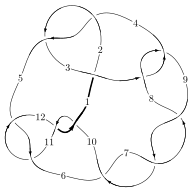
\includegraphics[width=112pt]{../../../GIT/diagram.site/Diagrams/png/919_12a_0118.png}\\
\ \ \ A knot diagram\footnotemark}&
\allowdisplaybreaks
\textbf{Linearized knot diagam} \\
\cline{2-2}
 &
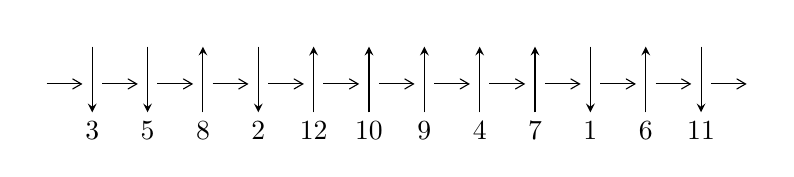
\begin{tikzpicture}[x=20pt, y=17pt]
	% nodes
	\node (C0) at (0, 0) {};
	\node (C1) at (1, 0) {};
	\node (C1U) at (1, +1) {};
	\node (C1D) at (1, -1) {3};

	\node (C2) at (2, 0) {};
	\node (C2U) at (2, +1) {};
	\node (C2D) at (2, -1) {5};

	\node (C3) at (3, 0) {};
	\node (C3U) at (3, +1) {};
	\node (C3D) at (3, -1) {8};

	\node (C4) at (4, 0) {};
	\node (C4U) at (4, +1) {};
	\node (C4D) at (4, -1) {2};

	\node (C5) at (5, 0) {};
	\node (C5U) at (5, +1) {};
	\node (C5D) at (5, -1) {12};

	\node (C6) at (6, 0) {};
	\node (C6U) at (6, +1) {};
	\node (C6D) at (6, -1) {10};

	\node (C7) at (7, 0) {};
	\node (C7U) at (7, +1) {};
	\node (C7D) at (7, -1) {9};

	\node (C8) at (8, 0) {};
	\node (C8U) at (8, +1) {};
	\node (C8D) at (8, -1) {4};

	\node (C9) at (9, 0) {};
	\node (C9U) at (9, +1) {};
	\node (C9D) at (9, -1) {7};

	\node (C10) at (10, 0) {};
	\node (C10U) at (10, +1) {};
	\node (C10D) at (10, -1) {1};

	\node (C11) at (11, 0) {};
	\node (C11U) at (11, +1) {};
	\node (C11D) at (11, -1) {6};

	\node (C12) at (12, 0) {};
	\node (C12U) at (12, +1) {};
	\node (C12D) at (12, -1) {11};
	\node (C13) at (13, 0) {};

	% arrows
	\draw[->,>={angle 60}]
	(C0) edge (C1) (C1) edge (C2) (C2) edge (C3) (C3) edge (C4) (C4) edge (C5) (C5) edge (C6) (C6) edge (C7) (C7) edge (C8) (C8) edge (C9) (C9) edge (C10) (C10) edge (C11) (C11) edge (C12) (C12) edge (C13) ;	\draw[->,>=stealth]
	(C1U) edge (C1D) (C2U) edge (C2D) (C3D) edge (C3U) (C4U) edge (C4D) (C5D) edge (C5U) (C6D) edge (C6U) (C7D) edge (C7U) (C8D) edge (C8U) (C9D) edge (C9U) (C10U) edge (C10D) (C11D) edge (C11U) (C12U) edge (C12D) ;
	\end{tikzpicture} \\
\hhline{~~} \\& 
\textbf{Solving Sequence} \\ \cline{2-2} 
 &
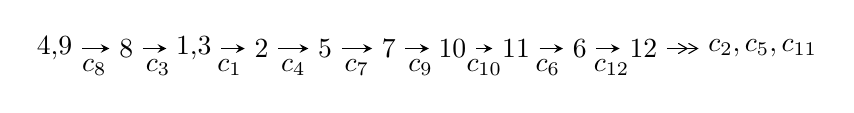
\begin{tikzpicture}[x=23pt, y=7pt]
	% node
	\node (A0) at (-1/8, 0) {4,9};
	\node (A1) at (1, 0) {8};
	\node (A2) at (33/16, 0) {1,3};
	\node (A3) at (25/8, 0) {2};
	\node (A4) at (33/8, 0) {5};
	\node (A5) at (41/8, 0) {7};
	\node (A6) at (49/8, 0) {10};
	\node (A7) at (57/8, 0) {11};
	\node (A8) at (65/8, 0) {6};
	\node (A9) at (73/8, 0) {12};
	\node (C1) at (1/2, -1) {$c_{8}$};
	\node (C2) at (3/2, -1) {$c_{3}$};
	\node (C3) at (21/8, -1) {$c_{1}$};
	\node (C4) at (29/8, -1) {$c_{4}$};
	\node (C5) at (37/8, -1) {$c_{7}$};
	\node (C6) at (45/8, -1) {$c_{9}$};
	\node (C7) at (53/8, -1) {$c_{10}$};
	\node (C8) at (61/8, -1) {$c_{6}$};
	\node (C9) at (69/8, -1) {$c_{12}$};
	\node (A10) at (11, 0) {$c_{2},c_{5},c_{11}$};

	% edge
	\draw[->,>=stealth]	
	(A0) edge (A1) (A1) edge (A2) (A2) edge (A3) (A3) edge (A4) (A4) edge (A5) (A5) edge (A6) (A6) edge (A7) (A7) edge (A8) (A8) edge (A9) ;
	\draw[->>,>={angle 60}]	
	(A9) edge (A10);
\end{tikzpicture} \\ 

\end{tabular} \\

\footnotetext{
The image of knot diagram is generated by the software ``\textbf{Draw programme}" developed by Andrew Bartholomew(\url{http://www.layer8.co.uk/maths/draw/index.htm\#Running-draw}), where we modified some parts for our purpose(\url{https://github.com/CATsTAILs/LinksPainter}).
}\phantom \\ \newline 
\centering \textbf{Ideals for irreducible components\footnotemark of $X_{\text{par}}$} 
 
\begin{align*}
I^u_{1}&=\langle 
4.88767\times10^{39} u^{69}-2.05229\times10^{38} u^{68}+\cdots+4.39249\times10^{39} b-2.55827\times10^{40},\\
\phantom{I^u_{1}}&\phantom{= \langle  }-8.11974\times10^{39} u^{69}+1.40212\times10^{39} u^{68}+\cdots+4.39249\times10^{39} a+6.03714\times10^{40},\;u^{70}- u^{69}+\cdots-12 u+4\rangle \\
\\
I^v_{1}&=\langle 
a,\;b- v-1,\;v^2+v+1\rangle \\
\end{align*}
\raggedright * 2 irreducible components of $\dim_{\mathbb{C}}=0$, with total 72 representations.\\
\footnotetext{All coefficients of polynomials are rational numbers. But the coefficients are sometimes approximated in decimal forms when there is not enough margin.}
\newpage
\renewcommand{\arraystretch}{1}
\centering \section*{I. $I^u_{1}= \langle 4.89\times10^{39} u^{69}-2.05\times10^{38} u^{68}+\cdots+4.39\times10^{39} b-2.56\times10^{40},\;-8.12\times10^{39} u^{69}+1.40\times10^{39} u^{68}+\cdots+4.39\times10^{39} a+6.04\times10^{40},\;u^{70}- u^{69}+\cdots-12 u+4 \rangle$}
\flushleft \textbf{(i) Arc colorings}\\
\begin{tabular}{m{7pt} m{180pt} m{7pt} m{180pt} }
\flushright $a_{4}=$&$\begin{pmatrix}0\\u\end{pmatrix}$ \\
\flushright $a_{9}=$&$\begin{pmatrix}1\\0\end{pmatrix}$ \\
\flushright $a_{8}=$&$\begin{pmatrix}1\\u^2\end{pmatrix}$ \\
\flushright $a_{1}=$&$\begin{pmatrix}1.84855 u^{69}-0.319208 u^{68}+\cdots+27.0154 u-13.7442\\-1.11273 u^{69}+0.0467228 u^{68}+\cdots-4.82981 u+5.82420\end{pmatrix}$ \\
\flushright $a_{3}=$&$\begin{pmatrix}- u\\- u^3+u\end{pmatrix}$ \\
\flushright $a_{2}=$&$\begin{pmatrix}1.48418 u^{69}+0.111209 u^{68}+\cdots+23.4623 u-12.2083\\-0.723651 u^{69}+0.0742162 u^{68}+\cdots+0.973362 u+4.02410\end{pmatrix}$ \\
\flushright $a_{5}=$&$\begin{pmatrix}-0.263656 u^{69}-0.120324 u^{68}+\cdots-11.2277 u+1.80266\\-1.58490 u^{69}+0.439531 u^{68}+\cdots-15.7877 u+11.9416\end{pmatrix}$ \\
\flushright $a_{7}=$&$\begin{pmatrix}- u^2+1\\u^2\end{pmatrix}$ \\
\flushright $a_{10}=$&$\begin{pmatrix}u^4- u^2+1\\- u^4\end{pmatrix}$ \\
\flushright $a_{11}=$&$\begin{pmatrix}0.0566762 u^{69}+0.669845 u^{68}+\cdots+13.0126 u-7.86292\\-0.888567 u^{69}-0.0370187 u^{68}+\cdots-13.3944 u+7.93011\end{pmatrix}$ \\
\flushright $a_{6}=$&$\begin{pmatrix}- u^6+u^4-2 u^2+1\\u^6+u^2\end{pmatrix}$ \\
\flushright $a_{12}=$&$\begin{pmatrix}0.233751 u^{69}+0.504289 u^{68}+\cdots+14.1968 u-7.56914\\-1.10374 u^{69}-0.0225465 u^{68}+\cdots-15.1789 u+8.49479\end{pmatrix}$\\&\end{tabular}
\flushleft \textbf{(ii) Obstruction class $= -1$}\\~\\
\flushleft \textbf{(iii) Cusp Shapes $= -5.10416 u^{69}+0.201729 u^{68}+\cdots-71.8492 u+42.8742$}\\~\\
\newpage\renewcommand{\arraystretch}{1}
\flushleft \textbf{(iv) u-Polynomials at the component}\newline \\
\begin{tabular}{m{50pt}|m{274pt}}
Crossings & \hspace{64pt}u-Polynomials at each crossing \\
\hline $$\begin{aligned}c_{1}\end{aligned}$$&$\begin{aligned}
&u^{70}+41 u^{69}+\cdots+8 u+1
\end{aligned}$\\
\hline $$\begin{aligned}c_{2},c_{4}\end{aligned}$$&$\begin{aligned}
&u^{70}-3 u^{69}+\cdots-4 u+1
\end{aligned}$\\
\hline $$\begin{aligned}c_{3},c_{8}\end{aligned}$$&$\begin{aligned}
&u^{70}+u^{69}+\cdots+12 u+4
\end{aligned}$\\
\hline $$\begin{aligned}c_{5},c_{11}\end{aligned}$$&$\begin{aligned}
&u^{70}+2 u^{69}+\cdots- u+1
\end{aligned}$\\
\hline $$\begin{aligned}c_{6},c_{7},c_{9}\end{aligned}$$&$\begin{aligned}
&u^{70}-15 u^{69}+\cdots-200 u+16
\end{aligned}$\\
\hline $$\begin{aligned}c_{10},c_{12}\end{aligned}$$&$\begin{aligned}
&u^{70}+26 u^{69}+\cdots+11 u+1
\end{aligned}$\\
\hline
\end{tabular}\\~\\
\newpage\renewcommand{\arraystretch}{1}
\flushleft \textbf{(v) Riley Polynomials at the component}\newline \\
\begin{tabular}{m{50pt}|m{274pt}}
Crossings & \hspace{64pt}Riley Polynomials at each crossing \\
\hline $$\begin{aligned}c_{1}\end{aligned}$$&$\begin{aligned}
&y^{70}-21 y^{69}+\cdots+32 y+1
\end{aligned}$\\
\hline $$\begin{aligned}c_{2},c_{4}\end{aligned}$$&$\begin{aligned}
&y^{70}-41 y^{69}+\cdots-8 y+1
\end{aligned}$\\
\hline $$\begin{aligned}c_{3},c_{8}\end{aligned}$$&$\begin{aligned}
&y^{70}-15 y^{69}+\cdots-200 y+16
\end{aligned}$\\
\hline $$\begin{aligned}c_{5},c_{11}\end{aligned}$$&$\begin{aligned}
&y^{70}+26 y^{69}+\cdots+11 y+1
\end{aligned}$\\
\hline $$\begin{aligned}c_{6},c_{7},c_{9}\end{aligned}$$&$\begin{aligned}
&y^{70}+77 y^{69}+\cdots+2272 y+256
\end{aligned}$\\
\hline $$\begin{aligned}c_{10},c_{12}\end{aligned}$$&$\begin{aligned}
&y^{70}+38 y^{69}+\cdots+131 y+1
\end{aligned}$\\
\hline
\end{tabular}\\~\\
\newpage\flushleft \textbf{(vi) Complex Volumes and Cusp Shapes}
$$\begin{array}{c|c|c}  
\text{Solutions to }I^u_{1}& \I (\text{vol} + \sqrt{-1}CS) & \text{Cusp shape}\\
 \hline 
\begin{aligned}
u &= -0.856012 + 0.547090 I \\
a &= -0.649388 + 0.664283 I \\
b &= \phantom{-}0.678669 - 1.019120 I\end{aligned}
 & -4.18862 - 5.65542 I & -4.40524 + 8.10333 I \\ \hline\begin{aligned}
u &= -0.856012 - 0.547090 I \\
a &= -0.649388 - 0.664283 I \\
b &= \phantom{-}0.678669 + 1.019120 I\end{aligned}
 & -4.18862 + 5.65542 I & -4.40524 - 8.10333 I \\ \hline\begin{aligned}
u &= -0.959078 + 0.338964 I \\
a &= \phantom{-}1.001140 - 0.104262 I \\
b &= -0.162521 - 0.081892 I\end{aligned}
 & \phantom{-}3.53851 - 0.96635 I & \phantom{-}7.82026 + 0. I\phantom{ +0.000000I} \\ \hline\begin{aligned}
u &= -0.959078 - 0.338964 I \\
a &= \phantom{-}1.001140 + 0.104262 I \\
b &= -0.162521 + 0.081892 I\end{aligned}
 & \phantom{-}3.53851 + 0.96635 I & \phantom{-}7.82026 + 0. I\phantom{ +0.000000I} \\ \hline\begin{aligned}
u &= -1.019040 + 0.052169 I \\
a &= \phantom{-}0.438523 - 0.219399 I \\
b &= -0.145309 - 0.850245 I\end{aligned}
 & \phantom{-}4.86369 + 0.47978 I & \phantom{-}8.80207 + 0. I\phantom{ +0.000000I} \\ \hline\begin{aligned}
u &= -1.019040 - 0.052169 I \\
a &= \phantom{-}0.438523 + 0.219399 I \\
b &= -0.145309 + 0.850245 I\end{aligned}
 & \phantom{-}4.86369 - 0.47978 I & \phantom{-}8.80207 + 0. I\phantom{ +0.000000I} \\ \hline\begin{aligned}
u &= \phantom{-}1.027600 + 0.119592 I \\
a &= -0.292337 - 0.225712 I \\
b &= \phantom{-}0.205304 - 0.936042 I\end{aligned}
 & \phantom{-}4.71065 + 4.96261 I & \phantom{-}8.04821 - 7.02524 I \\ \hline\begin{aligned}
u &= \phantom{-}1.027600 - 0.119592 I \\
a &= -0.292337 + 0.225712 I \\
b &= \phantom{-}0.205304 + 0.936042 I\end{aligned}
 & \phantom{-}4.71065 - 4.96261 I & \phantom{-}8.04821 + 7.02524 I \\ \hline\begin{aligned}
u &= -0.443664 + 0.844769 I \\
a &= -0.538375 + 0.337845 I \\
b &= -0.096708 - 0.471281 I\end{aligned}
 & -1.19762 + 5.98159 I & -0.92170 - 7.29563 I \\ \hline\begin{aligned}
u &= -0.443664 - 0.844769 I \\
a &= -0.538375 - 0.337845 I \\
b &= -0.096708 + 0.471281 I\end{aligned}
 & -1.19762 - 5.98159 I & -0.92170 + 7.29563 I\\
 \hline 
 \end{array}$$\newpage$$\begin{array}{c|c|c}  
\text{Solutions to }I^u_{1}& \I (\text{vol} + \sqrt{-1}CS) & \text{Cusp shape}\\
 \hline 
\begin{aligned}
u &= \phantom{-}0.971885 + 0.410627 I \\
a &= -1.096340 - 0.187273 I \\
b &= \phantom{-}0.241292 - 0.293397 I\end{aligned}
 & \phantom{-}2.85579 + 6.32679 I & \phantom{-0.000000 } 0 \\ \hline\begin{aligned}
u &= \phantom{-}0.971885 - 0.410627 I \\
a &= -1.096340 + 0.187273 I \\
b &= \phantom{-}0.241292 + 0.293397 I\end{aligned}
 & \phantom{-}2.85579 - 6.32679 I & \phantom{-0.000000 } 0 \\ \hline\begin{aligned}
u &= \phantom{-}0.839415 + 0.383054 I \\
a &= \phantom{-}0.167368 + 0.464643 I \\
b &= \phantom{-}0.014763 - 1.203170 I\end{aligned}
 & -0.17528 + 3.69433 I & \phantom{-}3.69302 - 7.55665 I \\ \hline\begin{aligned}
u &= \phantom{-}0.839415 - 0.383054 I \\
a &= \phantom{-}0.167368 - 0.464643 I \\
b &= \phantom{-}0.014763 + 1.203170 I\end{aligned}
 & -0.17528 - 3.69433 I & \phantom{-}3.69302 + 7.55665 I \\ \hline\begin{aligned}
u &= -0.610913 + 0.667828 I \\
a &= -1.309430 + 0.512503 I \\
b &= \phantom{-}0.409626 + 0.116110 I\end{aligned}
 & -5.02013 + 1.13894 I & -7.42078 - 0.58795 I \\ \hline\begin{aligned}
u &= -0.610913 - 0.667828 I \\
a &= -1.309430 - 0.512503 I \\
b &= \phantom{-}0.409626 - 0.116110 I\end{aligned}
 & -5.02013 - 1.13894 I & -7.42078 + 0.58795 I \\ \hline\begin{aligned}
u &= \phantom{-}1.007960 + 0.482476 I \\
a &= \phantom{-}0.671035 + 0.116495 I \\
b &= -0.043821 - 0.531729 I\end{aligned}
 & \phantom{-}1.70900 + 5.48430 I & \phantom{-0.000000 } 0 \\ \hline\begin{aligned}
u &= \phantom{-}1.007960 - 0.482476 I \\
a &= \phantom{-}0.671035 - 0.116495 I \\
b &= -0.043821 + 0.531729 I\end{aligned}
 & \phantom{-}1.70900 - 5.48430 I & \phantom{-0.000000 } 0 \\ \hline\begin{aligned}
u &= \phantom{-}0.367833 + 0.798582 I \\
a &= \phantom{-}0.547260 + 0.067881 I \\
b &= \phantom{-}0.238259 - 0.220293 I\end{aligned}
 & -0.434483 - 0.891477 I & \phantom{-}0.84820 + 1.91068 I \\ \hline\begin{aligned}
u &= \phantom{-}0.367833 - 0.798582 I \\
a &= \phantom{-}0.547260 - 0.067881 I \\
b &= \phantom{-}0.238259 + 0.220293 I\end{aligned}
 & -0.434483 + 0.891477 I & \phantom{-}0.84820 - 1.91068 I\\
 \hline 
 \end{array}$$\newpage$$\begin{array}{c|c|c}  
\text{Solutions to }I^u_{1}& \I (\text{vol} + \sqrt{-1}CS) & \text{Cusp shape}\\
 \hline 
\begin{aligned}
u &= \phantom{-}0.688189 + 0.495014 I \\
a &= -0.751143 - 0.485185 I \\
b &= \phantom{-}0.731991 + 0.183516 I\end{aligned}
 & -1.70612 + 1.90353 I & -1.29790 - 4.47310 I \\ \hline\begin{aligned}
u &= \phantom{-}0.688189 - 0.495014 I \\
a &= -0.751143 + 0.485185 I \\
b &= \phantom{-}0.731991 - 0.183516 I\end{aligned}
 & -1.70612 - 1.90353 I & -1.29790 + 4.47310 I \\ \hline\begin{aligned}
u &= -1.024030 + 0.531995 I \\
a &= -0.847273 + 0.128927 I \\
b &= \phantom{-}0.143783 - 0.298287 I\end{aligned}
 & \phantom{-}0.79072 - 10.96610 I & \phantom{-0.000000 } 0 \\ \hline\begin{aligned}
u &= -1.024030 - 0.531995 I \\
a &= -0.847273 - 0.128927 I \\
b &= \phantom{-}0.143783 + 0.298287 I\end{aligned}
 & \phantom{-}0.79072 + 10.96610 I & \phantom{-0.000000 } 0 \\ \hline\begin{aligned}
u &= -0.734851 + 0.407087 I \\
a &= -2.18354 + 0.39505 I \\
b &= -0.093179 + 0.722090 I\end{aligned}
 & -1.82583 - 3.75171 I & -0.39629 + 7.22205 I \\ \hline\begin{aligned}
u &= -0.734851 - 0.407087 I \\
a &= -2.18354 - 0.39505 I \\
b &= -0.093179 - 0.722090 I\end{aligned}
 & -1.82583 + 3.75171 I & -0.39629 - 7.22205 I \\ \hline\begin{aligned}
u &= -0.690889 + 0.415366 I \\
a &= -0.012282 + 0.905962 I \\
b &= -0.01931 - 1.84269 I\end{aligned}
 & -1.97137 + 0.49525 I & -1.21375 + 3.39141 I \\ \hline\begin{aligned}
u &= -0.690889 - 0.415366 I \\
a &= -0.012282 - 0.905962 I \\
b &= -0.01931 + 1.84269 I\end{aligned}
 & -1.97137 - 0.49525 I & -1.21375 - 3.39141 I \\ \hline\begin{aligned}
u &= \phantom{-}0.859252 + 0.847811 I \\
a &= -1.12334 - 1.09661 I \\
b &= \phantom{-}2.28142 - 0.13713 I\end{aligned}
 & -3.86556 + 1.55363 I & \phantom{-0.000000 } 0 \\ \hline\begin{aligned}
u &= \phantom{-}0.859252 - 0.847811 I \\
a &= -1.12334 + 1.09661 I \\
b &= \phantom{-}2.28142 + 0.13713 I\end{aligned}
 & -3.86556 - 1.55363 I & \phantom{-0.000000 } 0\\
 \hline 
 \end{array}$$\newpage$$\begin{array}{c|c|c}  
\text{Solutions to }I^u_{1}& \I (\text{vol} + \sqrt{-1}CS) & \text{Cusp shape}\\
 \hline 
\begin{aligned}
u &= -0.850893 + 0.884624 I \\
a &= \phantom{-}1.10267 - 1.18353 I \\
b &= -2.50998 + 0.01246 I\end{aligned}
 & -5.50548 + 3.78563 I & \phantom{-0.000000 } 0 \\ \hline\begin{aligned}
u &= -0.850893 - 0.884624 I \\
a &= \phantom{-}1.10267 + 1.18353 I \\
b &= -2.50998 - 0.01246 I\end{aligned}
 & -5.50548 - 3.78563 I & \phantom{-0.000000 } 0 \\ \hline\begin{aligned}
u &= -0.892645 + 0.859249 I \\
a &= -1.30636 + 1.71490 I \\
b &= \phantom{-}2.43773 + 0.22609 I\end{aligned}
 & -7.66688 - 0.08605 I & \phantom{-0.000000 } 0 \\ \hline\begin{aligned}
u &= -0.892645 - 0.859249 I \\
a &= -1.30636 - 1.71490 I \\
b &= \phantom{-}2.43773 - 0.22609 I\end{aligned}
 & -7.66688 + 0.08605 I & \phantom{-0.000000 } 0 \\ \hline\begin{aligned}
u &= -0.748791 + 0.124504 I \\
a &= \phantom{-}0.658521 - 0.117735 I \\
b &= -0.490170 + 0.349419 I\end{aligned}
 & \phantom{-}1.174050 - 0.188994 I & \phantom{-}9.05728 + 0.63012 I \\ \hline\begin{aligned}
u &= -0.748791 - 0.124504 I \\
a &= \phantom{-}0.658521 + 0.117735 I \\
b &= -0.490170 - 0.349419 I\end{aligned}
 & \phantom{-}1.174050 + 0.188994 I & \phantom{-}9.05728 - 0.63012 I \\ \hline\begin{aligned}
u &= -0.847834 + 0.919383 I \\
a &= -1.01430 + 1.70268 I \\
b &= \phantom{-}2.41082 - 0.49572 I\end{aligned}
 & -7.59275 + 3.10194 I & \phantom{-0.000000 } 0 \\ \hline\begin{aligned}
u &= -0.847834 - 0.919383 I \\
a &= -1.01430 - 1.70268 I \\
b &= \phantom{-}2.41082 + 0.49572 I\end{aligned}
 & -7.59275 - 3.10194 I & \phantom{-0.000000 } 0 \\ \hline\begin{aligned}
u &= \phantom{-}0.947471 + 0.820362 I \\
a &= -1.33084 - 1.01743 I \\
b &= \phantom{-}2.20960 - 0.80470 I\end{aligned}
 & -3.59203 + 4.66330 I & \phantom{-0.000000 } 0 \\ \hline\begin{aligned}
u &= \phantom{-}0.947471 - 0.820362 I \\
a &= -1.33084 + 1.01743 I \\
b &= \phantom{-}2.20960 + 0.80470 I\end{aligned}
 & -3.59203 - 4.66330 I & \phantom{-0.000000 } 0\\
 \hline 
 \end{array}$$\newpage$$\begin{array}{c|c|c}  
\text{Solutions to }I^u_{1}& \I (\text{vol} + \sqrt{-1}CS) & \text{Cusp shape}\\
 \hline 
\begin{aligned}
u &= \phantom{-}0.910528 + 0.864183 I \\
a &= \phantom{-}1.73727 + 1.07847 I \\
b &= -3.13501 + 0.34918 I\end{aligned}
 & -9.32357 + 0.88762 I & \phantom{-0.000000 } 0 \\ \hline\begin{aligned}
u &= \phantom{-}0.910528 - 0.864183 I \\
a &= \phantom{-}1.73727 - 1.07847 I \\
b &= -3.13501 - 0.34918 I\end{aligned}
 & -9.32357 - 0.88762 I & \phantom{-0.000000 } 0 \\ \hline\begin{aligned}
u &= -0.930113 + 0.845405 I \\
a &= -1.71742 + 0.97375 I \\
b &= \phantom{-}2.83461 + 0.49195 I\end{aligned}
 & -7.54935 - 6.24533 I & \phantom{-0.000000 } 0 \\ \hline\begin{aligned}
u &= -0.930113 - 0.845405 I \\
a &= -1.71742 - 0.97375 I \\
b &= \phantom{-}2.83461 - 0.49195 I\end{aligned}
 & -7.54935 + 6.24533 I & \phantom{-0.000000 } 0 \\ \hline\begin{aligned}
u &= \phantom{-}0.920205 + 0.860055 I \\
a &= \phantom{-}1.36723 + 1.80376 I \\
b &= -2.64509 + 0.40060 I\end{aligned}
 & -9.29275 + 5.50542 I & \phantom{-0.000000 } 0 \\ \hline\begin{aligned}
u &= \phantom{-}0.920205 - 0.860055 I \\
a &= \phantom{-}1.36723 - 1.80376 I \\
b &= -2.64509 - 0.40060 I\end{aligned}
 & -9.29275 - 5.50542 I & \phantom{-0.000000 } 0 \\ \hline\begin{aligned}
u &= -0.918074 + 0.869398 I \\
a &= \phantom{-}1.26727 - 1.14504 I \\
b &= -2.55438 - 0.51995 I\end{aligned}
 & -9.50690 - 3.21924 I & \phantom{-0.000000 } 0 \\ \hline\begin{aligned}
u &= -0.918074 - 0.869398 I \\
a &= \phantom{-}1.26727 + 1.14504 I \\
b &= -2.55438 + 0.51995 I\end{aligned}
 & -9.50690 + 3.21924 I & \phantom{-0.000000 } 0 \\ \hline\begin{aligned}
u &= \phantom{-}0.855164 + 0.943687 I \\
a &= \phantom{-}0.94923 + 1.77875 I \\
b &= -2.59048 - 0.67761 I\end{aligned}
 & -9.18918 - 8.56419 I & \phantom{-0.000000 } 0 \\ \hline\begin{aligned}
u &= \phantom{-}0.855164 - 0.943687 I \\
a &= \phantom{-}0.94923 - 1.77875 I \\
b &= -2.59048 + 0.67761 I\end{aligned}
 & -9.18918 + 8.56419 I & \phantom{-0.000000 } 0\\
 \hline 
 \end{array}$$\newpage$$\begin{array}{c|c|c}  
\text{Solutions to }I^u_{1}& \I (\text{vol} + \sqrt{-1}CS) & \text{Cusp shape}\\
 \hline 
\begin{aligned}
u &= \phantom{-}0.895190 + 0.908857 I \\
a &= \phantom{-}1.15254 + 1.83519 I \\
b &= -2.76109 - 0.15164 I\end{aligned}
 & -13.44380 - 1.53868 I & \phantom{-0.000000 } 0 \\ \hline\begin{aligned}
u &= \phantom{-}0.895190 - 0.908857 I \\
a &= \phantom{-}1.15254 - 1.83519 I \\
b &= -2.76109 + 0.15164 I\end{aligned}
 & -13.44380 + 1.53868 I & \phantom{-0.000000 } 0 \\ \hline\begin{aligned}
u &= -0.969783 + 0.836843 I \\
a &= \phantom{-}1.39145 - 1.05225 I \\
b &= -2.35136 - 0.97184 I\end{aligned}
 & -5.13123 - 10.16380 I & \phantom{-0.000000 } 0 \\ \hline\begin{aligned}
u &= -0.969783 - 0.836843 I \\
a &= \phantom{-}1.39145 + 1.05225 I \\
b &= -2.35136 + 0.97184 I\end{aligned}
 & -5.13123 + 10.16380 I & \phantom{-0.000000 } 0 \\ \hline\begin{aligned}
u &= \phantom{-}0.659724 + 0.283358 I \\
a &= \phantom{-}2.35512 + 0.08593 I \\
b &= \phantom{-}0.315252 + 0.457091 I\end{aligned}
 & -1.17058 - 1.08332 I & \phantom{-}2.65386 - 2.01895 I \\ \hline\begin{aligned}
u &= \phantom{-}0.659724 - 0.283358 I \\
a &= \phantom{-}2.35512 - 0.08593 I \\
b &= \phantom{-}0.315252 - 0.457091 I\end{aligned}
 & -1.17058 + 1.08332 I & \phantom{-}2.65386 + 2.01895 I \\ \hline\begin{aligned}
u &= -0.050359 + 0.716046 I \\
a &= \phantom{-}0.121117 - 0.635002 I \\
b &= \phantom{-}0.171445 + 0.650196 I\end{aligned}
 & \phantom{-}0.76923 - 2.33777 I & \phantom{-}2.89499 + 4.69130 I \\ \hline\begin{aligned}
u &= -0.050359 - 0.716046 I \\
a &= \phantom{-}0.121117 + 0.635002 I \\
b &= \phantom{-}0.171445 - 0.650196 I\end{aligned}
 & \phantom{-}0.76923 + 2.33777 I & \phantom{-}2.89499 - 4.69130 I \\ \hline\begin{aligned}
u &= \phantom{-}0.206898 + 0.671469 I \\
a &= -0.186235 - 0.643840 I \\
b &= \phantom{-}0.128642 + 0.779464 I\end{aligned}
 & \phantom{-}0.55234 - 2.49681 I & \phantom{-}1.97976 + 2.11018 I \\ \hline\begin{aligned}
u &= \phantom{-}0.206898 - 0.671469 I \\
a &= -0.186235 + 0.643840 I \\
b &= \phantom{-}0.128642 - 0.779464 I\end{aligned}
 & \phantom{-}0.55234 + 2.49681 I & \phantom{-}1.97976 - 2.11018 I\\
 \hline 
 \end{array}$$\newpage$$\begin{array}{c|c|c}  
\text{Solutions to }I^u_{1}& \I (\text{vol} + \sqrt{-1}CS) & \text{Cusp shape}\\
 \hline 
\begin{aligned}
u &= \phantom{-}0.959789 + 0.876252 I \\
a &= \phantom{-}1.88469 + 0.94024 I \\
b &= -3.04179 + 0.99068 I\end{aligned}
 & -13.2339 + 8.1232 I & \phantom{-0.000000 } 0 \\ \hline\begin{aligned}
u &= \phantom{-}0.959789 - 0.876252 I \\
a &= \phantom{-}1.88469 - 0.94024 I \\
b &= -3.04179 - 0.99068 I\end{aligned}
 & -13.2339 - 8.1232 I & \phantom{-0.000000 } 0 \\ \hline\begin{aligned}
u &= -0.990634 + 0.851943 I \\
a &= -1.86694 + 0.78225 I \\
b &= \phantom{-}2.57901 + 1.20339 I\end{aligned}
 & -7.13528 - 9.63342 I & \phantom{-0.000000 } 0 \\ \hline\begin{aligned}
u &= -0.990634 - 0.851943 I \\
a &= -1.86694 - 0.78225 I \\
b &= \phantom{-}2.57901 - 1.20339 I\end{aligned}
 & -7.13528 + 9.63342 I & \phantom{-0.000000 } 0 \\ \hline\begin{aligned}
u &= \phantom{-}1.002140 + 0.866479 I \\
a &= \phantom{-}1.94196 + 0.77269 I \\
b &= -2.66868 + 1.42802 I\end{aligned}
 & -8.7104 + 15.2194 I & \phantom{-0.000000 } 0 \\ \hline\begin{aligned}
u &= \phantom{-}1.002140 - 0.866479 I \\
a &= \phantom{-}1.94196 - 0.77269 I \\
b &= -2.66868 - 1.42802 I\end{aligned}
 & -8.7104 - 15.2194 I & \phantom{-0.000000 } 0 \\ \hline\begin{aligned}
u &= \phantom{-}0.635965 + 0.105400 I \\
a &= -0.744808 + 0.354776 I \\
b &= \phantom{-}1.18138 - 0.88640 I\end{aligned}
 & -0.93204 + 2.71089 I & \phantom{-}3.68951 - 7.69678 I \\ \hline\begin{aligned}
u &= \phantom{-}0.635965 - 0.105400 I \\
a &= -0.744808 - 0.354776 I \\
b &= \phantom{-}1.18138 + 0.88640 I\end{aligned}
 & -0.93204 - 2.71089 I & \phantom{-}3.68951 + 7.69678 I \\ \hline\begin{aligned}
u &= \phantom{-}0.282390 + 0.481929 I \\
a &= \phantom{-}1.21593 - 0.82030 I \\
b &= \phantom{-}0.095269 + 0.174525 I\end{aligned}
 & -1.68308 - 0.59288 I & -4.15264 + 0.08163 I \\ \hline\begin{aligned}
u &= \phantom{-}0.282390 - 0.481929 I \\
a &= \phantom{-}1.21593 + 0.82030 I \\
b &= \phantom{-}0.095269 - 0.174525 I\end{aligned}
 & -1.68308 + 0.59288 I & -4.15264 - 0.08163 I\\
 \hline 
 \end{array}$$\newpage\newpage\renewcommand{\arraystretch}{1}
\centering \section*{II. $I^v_{1}= \langle a,\;b- v-1,\;v^2+v+1 \rangle$}
\flushleft \textbf{(i) Arc colorings}\\
\begin{tabular}{m{7pt} m{180pt} m{7pt} m{180pt} }
\flushright $a_{4}=$&$\begin{pmatrix}v\\0\end{pmatrix}$ \\
\flushright $a_{9}=$&$\begin{pmatrix}1\\0\end{pmatrix}$ \\
\flushright $a_{8}=$&$\begin{pmatrix}1\\0\end{pmatrix}$ \\
\flushright $a_{1}=$&$\begin{pmatrix}0\\v+1\end{pmatrix}$ \\
\flushright $a_{3}=$&$\begin{pmatrix}v\\0\end{pmatrix}$ \\
\flushright $a_{2}=$&$\begin{pmatrix}v\\v+1\end{pmatrix}$ \\
\flushright $a_{5}=$&$\begin{pmatrix}0\\- v-1\end{pmatrix}$ \\
\flushright $a_{7}=$&$\begin{pmatrix}1\\0\end{pmatrix}$ \\
\flushright $a_{10}=$&$\begin{pmatrix}1\\0\end{pmatrix}$ \\
\flushright $a_{11}=$&$\begin{pmatrix}1\\v\end{pmatrix}$ \\
\flushright $a_{6}=$&$\begin{pmatrix}1\\0\end{pmatrix}$ \\
\flushright $a_{12}=$&$\begin{pmatrix}v+1\\v\end{pmatrix}$\\&\end{tabular}
\flushleft \textbf{(ii) Obstruction class $= 1$}\\~\\
\flushleft \textbf{(iii) Cusp Shapes $= 4 v-1$}\\~\\
\newpage\renewcommand{\arraystretch}{1}
\flushleft \textbf{(iv) u-Polynomials at the component}\newline \\
\begin{tabular}{m{50pt}|m{274pt}}
Crossings & \hspace{64pt}u-Polynomials at each crossing \\
\hline $$\begin{aligned}c_{1},c_{2}\end{aligned}$$&$\begin{aligned}
&(u-1)^2
\end{aligned}$\\
\hline $$\begin{aligned}c_{3},c_{6},c_{7}\\c_{8},c_{9}\end{aligned}$$&$\begin{aligned}
&u^2
\end{aligned}$\\
\hline $$\begin{aligned}c_{4}\end{aligned}$$&$\begin{aligned}
&(u+1)^2
\end{aligned}$\\
\hline $$\begin{aligned}c_{5},c_{12}\end{aligned}$$&$\begin{aligned}
&u^2+u+1
\end{aligned}$\\
\hline $$\begin{aligned}c_{10},c_{11}\end{aligned}$$&$\begin{aligned}
&u^2- u+1
\end{aligned}$\\
\hline
\end{tabular}\\~\\
\newpage\renewcommand{\arraystretch}{1}
\flushleft \textbf{(v) Riley Polynomials at the component}\newline \\
\begin{tabular}{m{50pt}|m{274pt}}
Crossings & \hspace{64pt}Riley Polynomials at each crossing \\
\hline $$\begin{aligned}c_{1},c_{2},c_{4}\end{aligned}$$&$\begin{aligned}
&(y-1)^2
\end{aligned}$\\
\hline $$\begin{aligned}c_{3},c_{6},c_{7}\\c_{8},c_{9}\end{aligned}$$&$\begin{aligned}
&y^2
\end{aligned}$\\
\hline $$\begin{aligned}c_{5},c_{10},c_{11}\\c_{12}\end{aligned}$$&$\begin{aligned}
&y^2+y+1
\end{aligned}$\\
\hline
\end{tabular}\\~\\
\newpage\flushleft \textbf{(vi) Complex Volumes and Cusp Shapes}
$$\begin{array}{c|c|c}  
\text{Solutions to }I^v_{1}& \I (\text{vol} + \sqrt{-1}CS) & \text{Cusp shape}\\
 \hline 
\begin{aligned}
v &= -0.500000 + 0.866025 I \\
a &= \phantom{-0.000000 } 0 \\
b &= \phantom{-}0.500000 + 0.866025 I\end{aligned}
 & -1.64493 - 2.02988 I & -3.00000 + 3.46410 I \\ \hline\begin{aligned}
v &= -0.500000 - 0.866025 I \\
a &= \phantom{-0.000000 } 0 \\
b &= \phantom{-}0.500000 - 0.866025 I\end{aligned}
 & -1.64493 + 2.02988 I & -3.00000 - 3.46410 I\\
 \hline 
 \end{array}$$\newpage
\newpage\renewcommand{\arraystretch}{1}
\centering \section*{ III. u-Polynomials}
\begin{tabular}{m{50pt}|m{274pt}}
Crossings & \hspace{64pt}u-Polynomials at each crossing \\
\hline $$\begin{aligned}c_{1}\end{aligned}$$&$\begin{aligned}
&((u-1)^2)(u^{70}+41 u^{69}+\cdots+8 u+1)
\end{aligned}$\\
\hline $$\begin{aligned}c_{2}\end{aligned}$$&$\begin{aligned}
&((u-1)^2)(u^{70}-3 u^{69}+\cdots-4 u+1)
\end{aligned}$\\
\hline $$\begin{aligned}c_{3},c_{8}\end{aligned}$$&$\begin{aligned}
&u^2(u^{70}+u^{69}+\cdots+12 u+4)
\end{aligned}$\\
\hline $$\begin{aligned}c_{4}\end{aligned}$$&$\begin{aligned}
&((u+1)^2)(u^{70}-3 u^{69}+\cdots-4 u+1)
\end{aligned}$\\
\hline $$\begin{aligned}c_{5}\end{aligned}$$&$\begin{aligned}
&(u^2+u+1)(u^{70}+2 u^{69}+\cdots- u+1)
\end{aligned}$\\
\hline $$\begin{aligned}c_{6},c_{7},c_{9}\end{aligned}$$&$\begin{aligned}
&u^2(u^{70}-15 u^{69}+\cdots-200 u+16)
\end{aligned}$\\
\hline $$\begin{aligned}c_{10}\end{aligned}$$&$\begin{aligned}
&(u^2- u+1)(u^{70}+26 u^{69}+\cdots+11 u+1)
\end{aligned}$\\
\hline $$\begin{aligned}c_{11}\end{aligned}$$&$\begin{aligned}
&(u^2- u+1)(u^{70}+2 u^{69}+\cdots- u+1)
\end{aligned}$\\
\hline $$\begin{aligned}c_{12}\end{aligned}$$&$\begin{aligned}
&(u^2+u+1)(u^{70}+26 u^{69}+\cdots+11 u+1)
\end{aligned}$\\
\hline
\end{tabular}\newpage\renewcommand{\arraystretch}{1}
\centering \section*{ IV. Riley Polynomials}
\begin{tabular}{m{50pt}|m{274pt}}
Crossings & \hspace{64pt}Riley Polynomials at each crossing \\
\hline $$\begin{aligned}c_{1}\end{aligned}$$&$\begin{aligned}
&((y-1)^2)(y^{70}-21 y^{69}+\cdots+32 y+1)
\end{aligned}$\\
\hline $$\begin{aligned}c_{2},c_{4}\end{aligned}$$&$\begin{aligned}
&((y-1)^2)(y^{70}-41 y^{69}+\cdots-8 y+1)
\end{aligned}$\\
\hline $$\begin{aligned}c_{3},c_{8}\end{aligned}$$&$\begin{aligned}
&y^2(y^{70}-15 y^{69}+\cdots-200 y+16)
\end{aligned}$\\
\hline $$\begin{aligned}c_{5},c_{11}\end{aligned}$$&$\begin{aligned}
&(y^2+y+1)(y^{70}+26 y^{69}+\cdots+11 y+1)
\end{aligned}$\\
\hline $$\begin{aligned}c_{6},c_{7},c_{9}\end{aligned}$$&$\begin{aligned}
&y^2(y^{70}+77 y^{69}+\cdots+2272 y+256)
\end{aligned}$\\
\hline $$\begin{aligned}c_{10},c_{12}\end{aligned}$$&$\begin{aligned}
&(y^2+y+1)(y^{70}+38 y^{69}+\cdots+131 y+1)
\end{aligned}$\\
\hline
\end{tabular}
\vskip 2pc
\end{document}